\documentclass[tikz]{standalone}
\usetikzlibrary{plotmarks}
\begin{document}

\begin{tikzpicture}
  \draw plot[mark=*] coordinates {(1,0)};
\end{tikzpicture}

\begin{tikzpicture}
  \draw[draw=blue, fill=yellow, line width=0.8pt, mark color=red] plot[mark=*, mark size=3.5pt] coordinates {(1,0)};
\end{tikzpicture}

\begin{tikzpicture}
  \draw[red] plot[mark=*, mark size=2.5pt, mark options={rotate=30, xscale=1.5, fill=orange, mark color=none, ball color=green, line width=0.6pt}] coordinates {(1,0)};
\end{tikzpicture}

\begin{tikzpicture}
  \draw[xscale=2, rotate=20, dashed] plot[mark=*] coordinates {(1,0)};
\end{tikzpicture}
\begin{tikzpicture}
  \draw plot[mark=x] coordinates {(1,0)};
\end{tikzpicture}

\begin{tikzpicture}
  \draw[draw=blue, fill=yellow, line width=0.8pt, mark color=red] plot[mark=x, mark size=3.5pt] coordinates {(1,0)};
\end{tikzpicture}
\begin{tikzpicture}
  \draw[red] plot[mark=x, mark size=2.5pt, mark options={rotate=30, xscale=1.5, fill=orange, mark color=none, ball color=green, line width=0.6pt}] coordinates {(1,0)};
\end{tikzpicture}
\begin{tikzpicture}
  \draw[xscale=2, rotate=20, dashed] plot[mark=x] coordinates {(1,0)};
\end{tikzpicture}
\begin{tikzpicture}
  \draw plot[mark=+] coordinates {(1,0)};
\end{tikzpicture}
\begin{tikzpicture}
  \draw[draw=blue, fill=yellow, line width=0.8pt, mark color=red] plot[mark=+, mark size=3.5pt] coordinates {(1,0)};
\end{tikzpicture}

\begin{tikzpicture}
  \draw[red] plot[mark=+, mark size=2.5pt, mark options={rotate=30, xscale=1.5, fill=orange, mark color=none, ball color=green, line width=0.6pt}] coordinates {(1,0)};
\end{tikzpicture}
\begin{tikzpicture}
  \draw[xscale=2, rotate=20, dashed] plot[mark=+] coordinates {(1,0)};
\end{tikzpicture}
\begin{tikzpicture}
  \draw plot[mark=-] coordinates {(1,0)};
\end{tikzpicture}
\begin{tikzpicture}
  \draw[draw=blue, fill=yellow, line width=0.8pt, mark color=red] plot[mark=-, mark size=3.5pt] coordinates {(1,0)};
\end{tikzpicture}
\begin{tikzpicture}
  \draw[red] plot[mark=-, mark size=2.5pt, mark options={rotate=30, xscale=1.5, fill=orange, mark color=none, ball color=green, line width=0.6pt}] coordinates {(1,0)};
\end{tikzpicture}
\begin{tikzpicture}
  \draw[xscale=2, rotate=20, dashed] plot[mark=-] coordinates {(1,0)};
\end{tikzpicture}
\begin{tikzpicture}
  \draw plot[mark=|] coordinates {(1,0)};
\end{tikzpicture}
\begin{tikzpicture}
  \draw[draw=blue, fill=yellow, line width=0.8pt, mark color=red] plot[mark=|, mark size=3.5pt] coordinates {(1,0)};
\end{tikzpicture}
\begin{tikzpicture}
  \draw[red] plot[mark=|, mark size=2.5pt, mark options={rotate=30, xscale=1.5, fill=orange, mark color=none, ball color=green, line width=0.6pt}] coordinates {(1,0)};
\end{tikzpicture}
\begin{tikzpicture}
  \draw[xscale=2, rotate=20, dashed] plot[mark=|] coordinates {(1,0)};
\end{tikzpicture}
\begin{tikzpicture}
  \draw plot[mark=o] coordinates {(1,0)};
\end{tikzpicture}

\begin{tikzpicture}
  \draw[draw=blue, fill=yellow, line width=0.8pt, mark color=red] plot[mark=o, mark size=3.5pt] coordinates {(1,0)};
\end{tikzpicture}

\begin{tikzpicture}
  \draw[red] plot[mark=o, mark size=2.5pt, mark options={rotate=30, xscale=1.5, fill=orange, mark color=none, ball color=green, line width=0.6pt}] coordinates {(1,0)};
\end{tikzpicture}
\begin{tikzpicture}
  \draw[xscale=2, rotate=20, dashed] plot[mark=o] coordinates {(1,0)};
\end{tikzpicture}
\begin{tikzpicture}
  \draw plot[mark=asterisk] coordinates {(1,0)};
\end{tikzpicture}

\begin{tikzpicture}
  \draw[draw=blue, fill=yellow, line width=0.8pt, mark color=red] plot[mark=asterisk, mark size=3.5pt] coordinates {(1,0)};
\end{tikzpicture}

\begin{tikzpicture}
  \draw[red] plot[mark=asterisk, mark size=2.5pt, mark options={rotate=30, xscale=1.5, fill=orange, mark color=none, ball color=green, line width=0.6pt}] coordinates {(1,0)};
\end{tikzpicture}
\begin{tikzpicture}
  \draw[xscale=2, rotate=20, dashed] plot[mark=asterisk] coordinates {(1,0)};
\end{tikzpicture}
\begin{tikzpicture}
  \draw plot[mark=star] coordinates {(1,0)};
\end{tikzpicture}

\begin{tikzpicture}
  \draw[draw=blue, fill=yellow, line width=0.8pt, mark color=red] plot[mark=star, mark size=3.5pt] coordinates {(1,0)};
\end{tikzpicture}

\begin{tikzpicture}
  \draw[red] plot[mark=star, mark size=2.5pt, mark options={rotate=30, xscale=1.5, fill=orange, mark color=none, ball color=green, line width=0.6pt}] coordinates {(1,0)};
\end{tikzpicture}
\begin{tikzpicture}
  \draw[xscale=2, rotate=20, dashed] plot[mark=star] coordinates {(1,0)};
\end{tikzpicture}

\begin{tikzpicture}
  \draw plot[mark=10-pointed star] coordinates {(1,0)};
\end{tikzpicture}

\begin{tikzpicture}
  \draw[draw=blue, fill=yellow, line width=0.8pt, mark color=red] plot[mark=10-pointed star, mark size=3.5pt] coordinates {(1,0)};
\end{tikzpicture}

\begin{tikzpicture}
  \draw[red] plot[mark=10-pointed star, mark size=2.5pt, mark options={rotate=30, xscale=1.5, fill=orange, mark color=none, ball color=green, line width=0.6pt}] coordinates {(1,0)};
\end{tikzpicture}

\begin{tikzpicture}
  \draw[xscale=2, rotate=20, dashed] plot[mark=10-pointed star] coordinates {(1,0)};
\end{tikzpicture}

\begin{tikzpicture}
  \draw plot[mark=oplus] coordinates {(1,0)};
\end{tikzpicture}

\begin{tikzpicture}
  \draw[draw=blue, fill=yellow, line width=0.8pt, mark color=red] plot[mark=oplus, mark size=3.5pt] coordinates {(1,0)};
\end{tikzpicture}

\begin{tikzpicture}
  \draw[red] plot[mark=oplus, mark size=2.5pt, mark options={rotate=30, xscale=1.5, fill=orange, mark color=none, ball color=green, line width=0.6pt}] coordinates {(1,0)};
\end{tikzpicture}

\begin{tikzpicture}
  \draw[xscale=2, rotate=20, dashed] plot[mark=oplus] coordinates {(1,0)};
\end{tikzpicture}

\begin{tikzpicture}
  \draw plot[mark=oplus*] coordinates {(1,0)};
\end{tikzpicture}

\begin{tikzpicture}
  \draw[draw=blue, fill=yellow, line width=0.8pt, mark color=red] plot[mark=oplus*, mark size=3.5pt] coordinates {(1,0)};
\end{tikzpicture}

\begin{tikzpicture}
  \draw[red] plot[mark=oplus*, mark size=2.5pt, mark options={rotate=30, xscale=1.5, fill=orange, mark color=none, ball color=green, line width=0.6pt}] coordinates {(1,0)};
\end{tikzpicture}

\begin{tikzpicture}
  \draw[xscale=2, rotate=20, dashed] plot[mark=oplus*] coordinates {(1,0)};
\end{tikzpicture}

\begin{tikzpicture}
  \draw plot[mark=otimes] coordinates {(1,0)};
\end{tikzpicture}

\begin{tikzpicture}
  \draw[draw=blue, fill=yellow, line width=0.8pt, mark color=red] plot[mark=otimes, mark size=3.5pt] coordinates {(1,0)};
\end{tikzpicture}

\begin{tikzpicture}
  \draw[red] plot[mark=otimes, mark size=2.5pt, mark options={rotate=30, xscale=1.5, fill=orange, mark color=none, ball color=green, line width=0.6pt}] coordinates {(1,0)};
\end{tikzpicture}
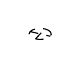
\begin{tikzpicture}
  \draw[xscale=2, rotate=20, dashed] plot[mark=otimes] coordinates {(1,0)};
\end{tikzpicture}

\begin{tikzpicture}
  \draw plot[mark=otimes*] coordinates {(1,0)};
\end{tikzpicture}

\begin{tikzpicture}
  \draw[draw=blue, fill=yellow, line width=0.8pt, mark color=red] plot[mark=otimes*, mark size=3.5pt] coordinates {(1,0)};
\end{tikzpicture}
\begin{tikzpicture}
  \draw[red] plot[mark=otimes*, mark size=2.5pt, mark options={rotate=30, xscale=1.5, fill=orange, mark color=none, ball color=green, line width=0.6pt}] coordinates {(1,0)};
\end{tikzpicture}
\begin{tikzpicture}
  \draw[xscale=2, rotate=20, dashed] plot[mark=otimes*] coordinates {(1,0)};
\end{tikzpicture}
\begin{tikzpicture}
  \draw plot[mark=square] coordinates {(1,0)};
\end{tikzpicture}
\begin{tikzpicture}
  \draw[draw=blue, fill=yellow, line width=0.8pt, mark color=red] plot[mark=square, mark size=3.5pt] coordinates {(1,0)};
\end{tikzpicture}
\begin{tikzpicture}
  \draw[red] plot[mark=square, mark size=2.5pt, mark options={rotate=30, xscale=1.5, fill=orange, mark color=none, ball color=green, line width=0.6pt}] coordinates {(1,0)};
\end{tikzpicture}
\begin{tikzpicture}
  \draw[xscale=2, rotate=20, dashed] plot[mark=square] coordinates {(1,0)};
\end{tikzpicture}
\begin{tikzpicture}
  \draw plot[mark=square*] coordinates {(1,0)};
\end{tikzpicture}
\begin{tikzpicture}
  \draw[draw=blue, fill=yellow, line width=0.8pt, mark color=red] plot[mark=square*, mark size=3.5pt] coordinates {(1,0)};
\end{tikzpicture}
\begin{tikzpicture}
  \draw[red] plot[mark=square*, mark size=2.5pt, mark options={rotate=30, xscale=1.5, fill=orange, mark color=none, ball color=green, line width=0.6pt}] coordinates {(1,0)};
\end{tikzpicture}
\begin{tikzpicture}
  \draw[xscale=2, rotate=20, dashed] plot[mark=square*] coordinates {(1,0)};
\end{tikzpicture}
\begin{tikzpicture}
  \draw plot[mark=triangle] coordinates {(1,0)};
\end{tikzpicture}
\begin{tikzpicture}
  \draw[draw=blue, fill=yellow, line width=0.8pt, mark color=red] plot[mark=triangle, mark size=3.5pt] coordinates {(1,0)};
\end{tikzpicture}
\begin{tikzpicture}
  \draw[red] plot[mark=triangle, mark size=2.5pt, mark options={rotate=30, xscale=1.5, fill=orange, mark color=none, ball color=green, line width=0.6pt}] coordinates {(1,0)};
\end{tikzpicture}
\begin{tikzpicture}
  \draw[xscale=2, rotate=20, dashed] plot[mark=triangle] coordinates {(1,0)};
\end{tikzpicture}
\begin{tikzpicture}
  \draw plot[mark=triangle*] coordinates {(1,0)};
\end{tikzpicture}
\begin{tikzpicture}
  \draw[draw=blue, fill=yellow, line width=0.8pt, mark color=red] plot[mark=triangle*, mark size=3.5pt] coordinates {(1,0)};
\end{tikzpicture}
\begin{tikzpicture}
  \draw[red] plot[mark=triangle*, mark size=2.5pt, mark options={rotate=30, xscale=1.5, fill=orange, mark color=none, ball color=green, line width=0.6pt}] coordinates {(1,0)};
\end{tikzpicture}
\begin{tikzpicture}
  \draw[xscale=2, rotate=20, dashed] plot[mark=triangle*] coordinates {(1,0)};
\end{tikzpicture}
\begin{tikzpicture}
  \draw plot[mark=diamond] coordinates {(1,0)};
\end{tikzpicture}
\begin{tikzpicture}
  \draw[draw=blue, fill=yellow, line width=0.8pt, mark color=red] plot[mark=diamond, mark size=3.5pt] coordinates {(1,0)};
\end{tikzpicture}
\begin{tikzpicture}
  \draw[red] plot[mark=diamond, mark size=2.5pt, mark options={rotate=30, xscale=1.5, fill=orange, mark color=none, ball color=green, line width=0.6pt}] coordinates {(1,0)};
\end{tikzpicture}
\begin{tikzpicture}
  \draw[xscale=2, rotate=20, dashed] plot[mark=diamond] coordinates {(1,0)};
\end{tikzpicture}
\begin{tikzpicture}
  \draw plot[mark=diamond*] coordinates {(1,0)};
\end{tikzpicture}
\begin{tikzpicture}
  \draw[draw=blue, fill=yellow, line width=0.8pt, mark color=red] plot[mark=diamond*, mark size=3.5pt] coordinates {(1,0)};
\end{tikzpicture}
\begin{tikzpicture}
  \draw[red] plot[mark=diamond*, mark size=2.5pt, mark options={rotate=30, xscale=1.5, fill=orange, mark color=none, ball color=green, line width=0.6pt}] coordinates {(1,0)};
\end{tikzpicture}
\begin{tikzpicture}
  \draw[xscale=2, rotate=20, dashed] plot[mark=diamond*] coordinates {(1,0)};
\end{tikzpicture}
\begin{tikzpicture}
  \draw plot[mark=halfdiamond*] coordinates {(1,0)};
\end{tikzpicture}
\begin{tikzpicture}
  \draw[draw=blue, fill=yellow, line width=0.8pt, mark color=red] plot[mark=halfdiamond*, mark size=3.5pt] coordinates {(1,0)};
\end{tikzpicture}
\begin{tikzpicture}
  \draw[red] plot[mark=halfdiamond*, mark size=2.5pt, mark options={rotate=30, xscale=1.5, fill=orange, mark color=none, ball color=green, line width=0.6pt}] coordinates {(1,0)};
\end{tikzpicture}
\begin{tikzpicture}
  \draw[xscale=2, rotate=20, dashed] plot[mark=halfdiamond*] coordinates {(1,0)};
\end{tikzpicture}
\begin{tikzpicture}
  \draw plot[mark=halfsquare*] coordinates {(1,0)};
\end{tikzpicture}
\begin{tikzpicture}
  \draw[draw=blue, fill=yellow, line width=0.8pt, mark color=red] plot[mark=halfsquare*, mark size=3.5pt] coordinates {(1,0)};
\end{tikzpicture}
\begin{tikzpicture}
  \draw[red] plot[mark=halfsquare*, mark size=2.5pt, mark options={rotate=30, xscale=1.5, fill=orange, mark color=none, ball color=green, line width=0.6pt}] coordinates {(1,0)};
\end{tikzpicture}
\begin{tikzpicture}
  \draw[xscale=2, rotate=20, dashed] plot[mark=halfsquare*] coordinates {(1,0)};
\end{tikzpicture}
\begin{tikzpicture}
  \draw plot[mark=halfsquare right*] coordinates {(1,0)};
\end{tikzpicture}
\begin{tikzpicture}
  \draw[draw=blue, fill=yellow, line width=0.8pt, mark color=red] plot[mark=halfsquare right*, mark size=3.5pt] coordinates {(1,0)};
\end{tikzpicture}
\begin{tikzpicture}
  \draw[red] plot[mark=halfsquare right*, mark size=2.5pt, mark options={rotate=30, xscale=1.5, fill=orange, mark color=none, ball color=green, line width=0.6pt}] coordinates {(1,0)};
\end{tikzpicture}
\begin{tikzpicture}
  \draw[xscale=2, rotate=20, dashed] plot[mark=halfsquare right*] coordinates {(1,0)};
\end{tikzpicture}
\begin{tikzpicture}
  \draw plot[mark=halfsquare left*] coordinates {(1,0)};
\end{tikzpicture}
\begin{tikzpicture}
  \draw[draw=blue, fill=yellow, line width=0.8pt, mark color=red] plot[mark=halfsquare left*, mark size=3.5pt] coordinates {(1,0)};
\end{tikzpicture}
\begin{tikzpicture}
  \draw[red] plot[mark=halfsquare left*, mark size=2.5pt, mark options={rotate=30, xscale=1.5, fill=orange, mark color=none, ball color=green, line width=0.6pt}] coordinates {(1,0)};
\end{tikzpicture}
\begin{tikzpicture}
  \draw[xscale=2, rotate=20, dashed] plot[mark=halfsquare left*] coordinates {(1,0)};
\end{tikzpicture}
\begin{tikzpicture}
  \draw plot[mark=pentagon] coordinates {(1,0)};
\end{tikzpicture}
\begin{tikzpicture}
  \draw[draw=blue, fill=yellow, line width=0.8pt, mark color=red] plot[mark=pentagon, mark size=3.5pt] coordinates {(1,0)};
\end{tikzpicture}
\begin{tikzpicture}
  \draw[red] plot[mark=pentagon, mark size=2.5pt, mark options={rotate=30, xscale=1.5, fill=orange, mark color=none, ball color=green, line width=0.6pt}] coordinates {(1,0)};
\end{tikzpicture}
\begin{tikzpicture}
  \draw[xscale=2, rotate=20, dashed] plot[mark=pentagon] coordinates {(1,0)};
\end{tikzpicture}
\begin{tikzpicture}
  \draw plot[mark=pentagon*] coordinates {(1,0)};
\end{tikzpicture}
\begin{tikzpicture}
  \draw[draw=blue, fill=yellow, line width=0.8pt, mark color=red] plot[mark=pentagon*, mark size=3.5pt] coordinates {(1,0)};
\end{tikzpicture}
\begin{tikzpicture}
  \draw[red] plot[mark=pentagon*, mark size=2.5pt, mark options={rotate=30, xscale=1.5, fill=orange, mark color=none, ball color=green, line width=0.6pt}] coordinates {(1,0)};
\end{tikzpicture}
\begin{tikzpicture}
  \draw[xscale=2, rotate=20, dashed] plot[mark=pentagon*] coordinates {(1,0)};
\end{tikzpicture}
\begin{tikzpicture}
  \draw plot[mark=Mercedes star] coordinates {(1,0)};
\end{tikzpicture}
\begin{tikzpicture}
  \draw[draw=blue, fill=yellow, line width=0.8pt, mark color=red] plot[mark=Mercedes star, mark size=3.5pt] coordinates {(1,0)};
\end{tikzpicture}
\begin{tikzpicture}
  \draw[red] plot[mark=Mercedes star, mark size=2.5pt, mark options={rotate=30, xscale=1.5, fill=orange, mark color=none, ball color=green, line width=0.6pt}] coordinates {(1,0)};
\end{tikzpicture}
\begin{tikzpicture}
  \draw[xscale=2, rotate=20, dashed] plot[mark=Mercedes star] coordinates {(1,0)};
\end{tikzpicture}
\begin{tikzpicture}
  \draw plot[mark=Mercedes star flipped] coordinates {(1,0)};
\end{tikzpicture}
\begin{tikzpicture}
  \draw[draw=blue, fill=yellow, line width=0.8pt, mark color=red] plot[mark=Mercedes star flipped, mark size=3.5pt] coordinates {(1,0)};
\end{tikzpicture}
\begin{tikzpicture}
  \draw[red] plot[mark=Mercedes star flipped, mark size=2.5pt, mark options={rotate=30, xscale=1.5, fill=orange, mark color=none, ball color=green, line width=0.6pt}] coordinates {(1,0)};
\end{tikzpicture}
\begin{tikzpicture}
  \draw[xscale=2, rotate=20, dashed] plot[mark=Mercedes star flipped] coordinates {(1,0)};
\end{tikzpicture}
\begin{tikzpicture}
  \draw plot[mark=halfcircle] coordinates {(1,0)};
\end{tikzpicture}
\begin{tikzpicture}
  \draw[draw=blue, fill=yellow, line width=0.8pt, mark color=red] plot[mark=halfcircle, mark size=3.5pt] coordinates {(1,0)};
\end{tikzpicture}
\begin{tikzpicture}
  \draw[red] plot[mark=halfcircle, mark size=2.5pt, mark options={rotate=30, xscale=1.5, fill=orange, mark color=none, ball color=green, line width=0.6pt}] coordinates {(1,0)};
\end{tikzpicture}
\begin{tikzpicture}
  \draw[xscale=2, rotate=20, dashed] plot[mark=halfcircle] coordinates {(1,0)};
\end{tikzpicture}
\begin{tikzpicture}
  \draw plot[mark=halfcircle*] coordinates {(1,0)};
\end{tikzpicture}
\begin{tikzpicture}
  \draw[draw=blue, fill=yellow, line width=0.8pt, mark color=red] plot[mark=halfcircle*, mark size=3.5pt] coordinates {(1,0)};
\end{tikzpicture}
\begin{tikzpicture}
  \draw[red] plot[mark=halfcircle*, mark size=2.5pt, mark options={rotate=30, xscale=1.5, fill=orange, mark color=none, ball color=green, line width=0.6pt}] coordinates {(1,0)};
\end{tikzpicture}
\begin{tikzpicture}
  \draw[xscale=2, rotate=20, dashed] plot[mark=halfcircle*] coordinates {(1,0)};
\end{tikzpicture}
\begin{tikzpicture}
  \draw plot[mark=heart] coordinates {(1,0)};
\end{tikzpicture}
\begin{tikzpicture}
  \draw[draw=blue, fill=yellow, line width=0.8pt, mark color=red] plot[mark=heart, mark size=3.5pt] coordinates {(1,0)};
\end{tikzpicture}
\begin{tikzpicture}
  \draw[red] plot[mark=heart, mark size=2.5pt, mark options={rotate=30, xscale=1.5, fill=orange, mark color=none, ball color=green, line width=0.6pt}] coordinates {(1,0)};
\end{tikzpicture}
\begin{tikzpicture}
  \draw[xscale=2, rotate=20, dashed] plot[mark=heart] coordinates {(1,0)};
\end{tikzpicture}
\begin{tikzpicture}
  \draw plot[mark=ball] coordinates {(1,0)};
\end{tikzpicture}
\begin{tikzpicture}
  \draw[draw=blue, fill=yellow, line width=0.8pt, mark color=red] plot[mark=ball, mark size=3.5pt] coordinates {(1,0)};
\end{tikzpicture}
\begin{tikzpicture}
  \draw[red] plot[mark=ball, mark size=2.5pt, mark options={rotate=30, xscale=1.5, fill=orange, mark color=none, ball color=green, line width=0.6pt}] coordinates {(1,0)};
\end{tikzpicture}
\begin{tikzpicture}
  \draw[xscale=2, rotate=20, dashed] plot[mark=ball] coordinates {(1,0)};
\end{tikzpicture}
\end{document}
